\documentclass[12pt]{article}

\usepackage[polish]{babel}
\usepackage{csquotes}
\usepackage[a4paper,top=2.5cm,bottom=2.5cm,left=3cm,right=2cm]{geometry}
\usepackage{indentfirst}
% Useful packages
\usepackage{lipsum}
\usepackage{amsmath}
\usepackage{graphicx}
\usepackage[colorlinks=true, allcolors=blue]{hyperref}
\usepackage{float}
\usepackage{fontspec}
\setmainfont{Times New Roman}
\setlength{\parindent}{1.25cm}
\linespread{1.5}
\setlength{\parskip}{6pt}
\usepackage[sorting=none, style=nature]{biblatex}
\addbibresource{bibliography.bib}

\hypersetup{linkcolor=black}
\usepackage[all]{hypcap}
\addto\captionspolish{\renewcommand{\figurename}{Rys.}}
\addto\captionspolish{\renewcommand{\tablename}{Tab.}}
\renewcommand{\tableautorefname}{Tab.} % PS
\renewcommand{\figureautorefname}{Rys.} % PS
\renewcommand{\listfigurename}{Spis rysunków}
\renewcommand{\listtablename}{Spis tabel}

\newcommand{\image}[3][16cm]{
\begin{figure}[H]
    \centering
    \includegraphics[width=#1]{imgs/#2}
    \caption{#3}
    \label{img:#2}
\end{figure}
}

\begin{document}

\newpage
\clearpage
\tableofcontents

\newpage
\addcontentsline{toc}{section}{Wstęp}
\section*{Wstęp}
\textit{W tym miejscu należy umieścić wstęp opisujący dlaczego ten temat jest istotny oraz motywację studenta w jego wyborze. Poniżej przykład jak zacząć nawiązanie do dziedziny, tak aby nie zaczynać pracy od oklepanej frazy „W dzisiejszych czasach …”:}

Nauka programowania od zawsze uznawana była za bardzo trudne zadanie dla nowicjuszy. Podejmowane przez nich próby pisania kodu często kończyły się niepowodzeniem i szybką rezygnacją.

Techniki biometryczne pozwalają na ochronę zasobów na urządzeniach bez potrzeby wprowadzania pinów, haseł oraz skomplikowanych wzorów, które mogą zostać zapomniane lub przechwycone przez osoby postronne. Wystarczy przyłożyć palec, a urządzenie zostaje odblokowane w ułamku sekundy. Jest to rozwiązanie bardzo wygodne dla użytkowników.

Efektywna komunikacja jest czynnikiem koniecznym do zagwarantowania rozwoju, stabilizacji, jak i również bezpieczeństwa niezależnie od płaszczyzny, na której zachodzi. Aby można było mówić o sukcesie procesu informowania, należy szczegółowo przeanalizować domenę w jakiej ma ona zachodzi oraz wybrać właściwą metodę przesyłania danych.

\textit{Jak widać, w każdym przypadku akapit zaczął się od określenia jakiejś pozytywnej lub negatywnej strony związanej z tematem pracy. Pozwala to na łatwe rozwinięcie treści.}

\textit{Jeśli brakuje wam weny, to wstępie możecie poruszyć opis problemów związanych z tematem, zastosowanie danej technologii, badania rynkowe np. o wzrastającej popularności danej technologii.}

\textit{Poniżej przedstawiłem przykładowe zakończenia z motywacją:}

Na rynku dostępnych jest wiele modeli robotów edukacyjnych, jednak większość 
z nich jest bardzo droga lub trudno dostępna dla szkół. Istnieje więc potrzeba stworzenia optymalnego modelu, łatwego w obsłudze, a zarazem będącego w przystępnej cenie. 

Praca ta ma na celu przedstawienie i porównanie różnych technik analizy interfejsu użytkownika tak, aby to, co wydaje się być intuicyjne i proste dla konstruującego stronę programisty, faktycznie takim się stało dla odbiorcy – użytkownika owego produktu.

\textbf{Całość, razem z zakończeniem powinna mieścić się na jednej stronie.}
\newpage

\addcontentsline{toc}{section}{Cel i zakres pracy}
\section*{Cel i zakres pracy}
Celem pracy było coś tam.
\newpage

\section{Część teoretyczna}
\subsection{Rys historyczny}

Dziedzina tej pracy jaką jest przetwarzanie obrazów ma początki swojej historii wcześniej niż urządzenia które obecnie nazywamy komputerami.

\subsubsection{Wywoływanie zdjęć}
Przetwarzanie obrazów to nie jest technologia, która mogła zacząć istnieć po wynalezieniu komputerów. Używając aparatów korzystających z kliszy filmowej, po ekspozycji należy go poddać procesowi wywoływania \autoref{fig:wywolywanie}. 
Polega on na wyciągnięciu pierwotnego efektu naświetlenia do obrazu, który oddaje scenę uchwyconą przez aparat \cite{doi:https://doi.org/10.1002/14356007.a20_001}. Proces w przypadku zdjęć aparatem na kliszę polega na zanurzaniu jej w odpowiednich związkach chemicznych na określone ilości czasu by otrzymać zamierzony efekt. 

\begin{figure}[H]
    \centering
    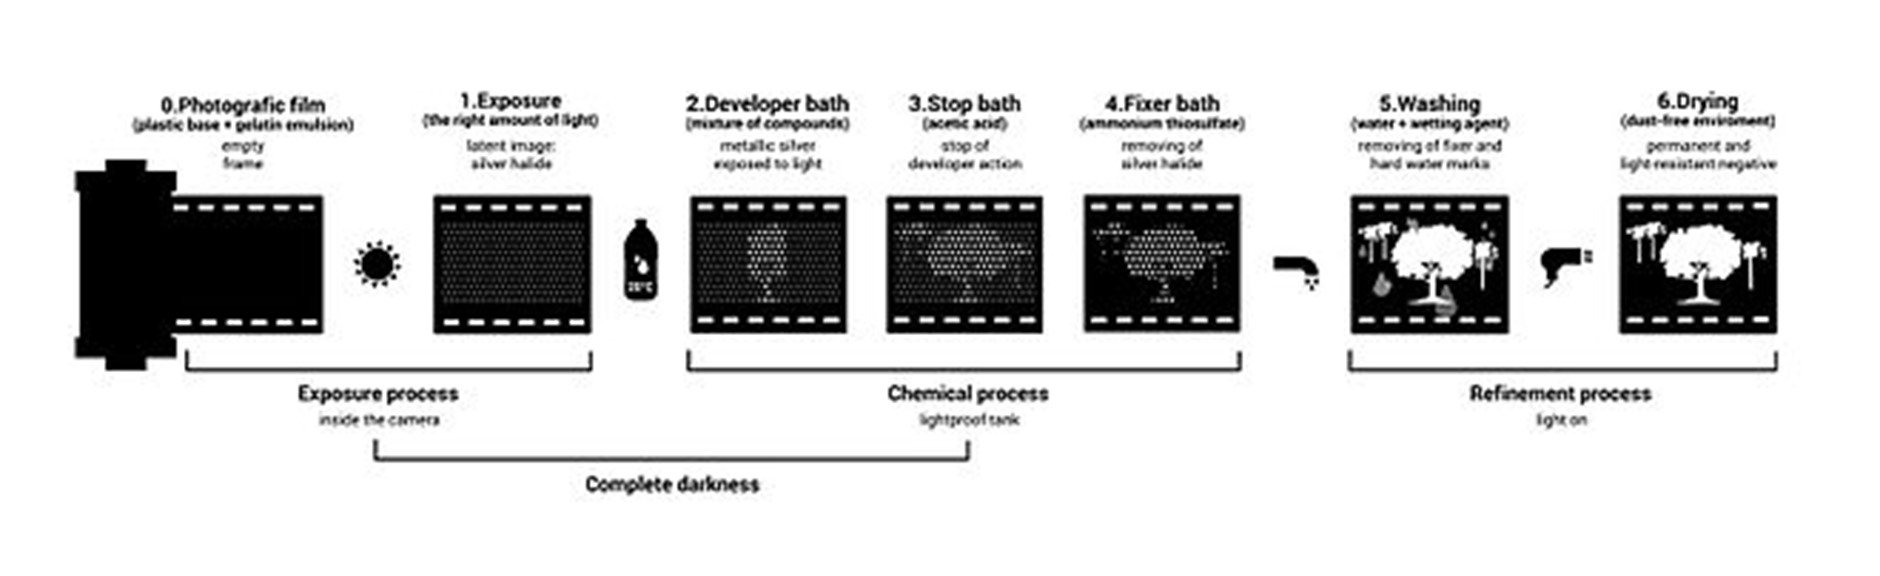
\includegraphics{./images/Picture1.jpg}
    \caption{Wywoływanie biało czarnej kliszy \cite{film}}.
    \label{fig:wywolywanie}
\end{figure}


Istnieją wariacje na temat takiego przetwarzania, różni się ono trochę w zależności od technologii kliszy. W niektórych przypadkach należy wywołać pozytyw zamiast negatywu \cite{almanac}. 
Następnie po wywoływaniu można poddać obróbce dalszymi chemikaliami jak np. siarczek sodu dla uzyskania efektu sepii \cite{sepia}. 

\subsubsection{Transmisja obrazów}
Technologia którą znamy dobrze w obecnych czasach powstała w latach 20. XX wieku dzięki pracy John Logie Baird'a \cite{times1926}. 
Zaprezentował on pierwszą na świecie transmisję telewizyjną na żywo.
W 1928 roku \cite{bairdCompany} firma założona przez niego emitowała też pierwsze nagranie przez atlantyk. 
Wszystko to dzięki przetwarzaniu analogowego sygnału video w celu zmniejszenia ilości danych potrzebnych do wyświetlenia obrazu w telewizji \cite{analogVideo}.

\subsubsection{Cyfrowe przetwarzanie obrazów}
Początki nowoczesnego przetwarzania obrazów zostały stworzone w latach 60. XX w. w Bell Laboratories, Jet Propulsion Laboratory, Massachusetts Institute of Technology i University of Maryland \cite{computerProcessing}. 
Początkowymi obszarami zastosowania były obrazy satelitarne, przesyłanie obrazów przez linie telefoniczne, diagnostyka obrazowa, wideofony, rozpoznawanie znaków i ulepszanie fotografii. 

Inicjalnie dużo skupiano się na ulepszeniu jakości obrazu. Pierwszym znaczącym użyciem tych technologii było mapowanie powierzchni księżyca za pomocą zdjęć z sondy kosmicznej w 1964 roku, gdzie naukowcy z Jet Propulsion Laboratory na podstawie tysięcy zdjęć odtworzyli powierzchnię księżyca. 
Przy następnej okazji mieli dostęp do 100000 zdjęć, na podstawie których mogli stworzyć mapę topograficzną, mapę kolorową oraz panoramiczną mozaikę księżyca, które przyczyniły się do pierwszego lądowania człowieka na księżycu \cite{digitalImageProcessing}.

Technologia ta jednak była ograniczona przez bardzo małe możliwości oraz trudną dostępność komputerów tamtych czasów. 
Wraz z ich rozwojem i wzrostem popularności cyfrowe przetwarzanie obrazów przestało być trudno dostępną dziedziną naukową i stopniowo zostało wdrażane do naszego codziennego życia. 
Obecnie około 80\% populacji krajów rozwiniętych jest w posiadaniu smartfona \cite{smartphones}, który na swoim wyposażeniu ma kamerę cyfrową. 
Są one ograniczone poprzez fizyczny rozmiar matrycy oraz jakość soczewek, które mogą zmieścić się w telefonach komórkowych. 
Pomimo tego dzięki przetwarzaniu obrazów można uchwycić za ich pomocą imponujące zdjęcia \cite{pixel}. 
Nowoczesne telefony są w stanie zachować na zdjęciu nocnym detale które może być ciężko zobaczyć ludzkim okiem \cite{nightMode} przez szybkie łączenie wielu obrazów o różnych długościach ekspozycji, redukcji szumów i korekcji kolorów.  

\subsection{Przegląd istniejących rozwiązań}

\subsubsection{Photoshop}
\begin{figure}[H]
    \centering
    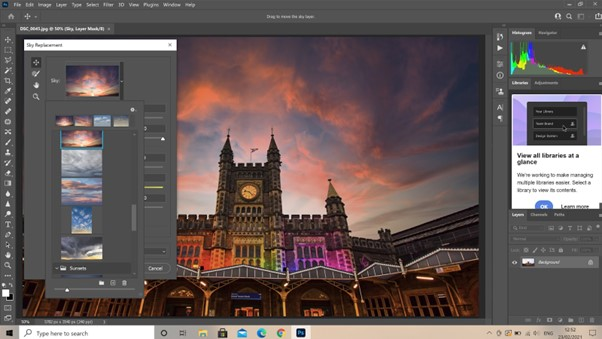
\includegraphics{./images/Picture2.jpg}
    \caption{Adobe Photoshop}
    \label{fig:photoshop}
\end{figure}

Wydany w 1990 roku do tworzenia i edytowania obrazów rastrowych jest jednym z najbardziej popularnych programów, a jego nazwa przedarła się do języka potocznego jako zamiennik dla fotomontażu. 
Użytkownikami tego oprogramowania są przeważnie artyści, fotografowie i twórcy internetowych memów. 
To narzędzie jest przystosowane do łatwości obsługi przez mniej zaawansowanych użytkowników i wszystko posiada przyjazny graficzny interfejs użytkownika. 

Funkcje, które pozwalają na przetwarzanie obrazów często nie odnoszą się bezpośrednio do operacji zawartych w znanych bibliotekach do przetwarzania obrazów. 
Ich obsługa jest uproszczona i przystosowana do bardziej artystycznych zastosowań. 
Bez zastosowania szczególnej ostrożności - jak tworzenie nowych warstw po każdej operacji lub częste zapisywanie kopii zapasowej obrazu – przetwarzanie obrazów często jest destruktywne, nie możemy odnieść się do dowolnego momentu w ciągu naszych operacji w celu dopasowania jej parametrów. 
Przetwarzanie innego obrazu za pomocą tego samego procesu jest problematyczne, gdyż wymaga to ciągłego śledzenia warstw. Wiele operacji trzeba powtórzyć indywidualnie ponieważ nie zapisujemy jej parametrów tylko rezultat poprzedniego wykonania. Wiele bardziej zaawansowanych procesów nie jest możliwych do zrealizowania za pomocą standardowych opcji dostępnych w programie. Historia operacji jest też ograniczona i nie można wyświetlić pełnej historii na jednym ekranie - można jedynie zamieniać stan aktualny na wcześniejszy.

\subsubsection{ImageJ}
\begin{figure}[H]
    \centering
    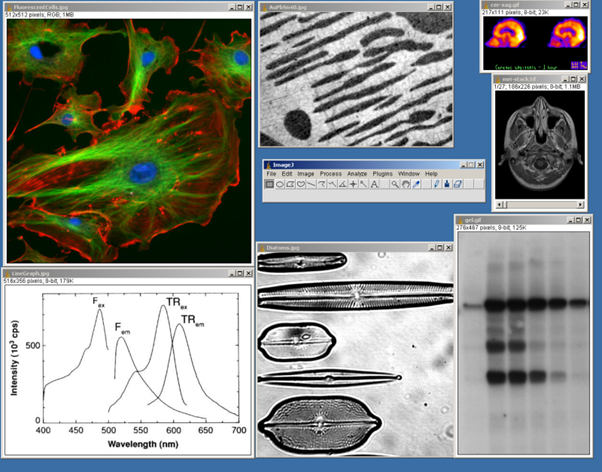
\includegraphics[width=0.8\linewidth]{./images/Picture3.png}
    \caption{ImageJ}
    \label{fig:imagej}
\end{figure}

Wydany w 1997 roku program ImageJ został wykonany przez National Institutes of Health, został tworzony podstawowo z zamiarem analizy obrazów w zastosowaniach medycznych. 
Odtwarza dokładnie wiele operacji z bibliotek do przetwarzania obrazów i kod aplikacji jest otwartoźródłowy - każdy może go zobaczyć, pomóc w rozwoju lub stworzyć własną wersję. 
Napisany został w języku Java i ma bardzo niskie wymagania sprzętowe jak na obecne czasy.

Program jest jednak przestarzały, mogą pojawić się problemy z uruchomieniem na nowszych systemach. Interfejs użytkownika wygląda archaicznie oraz jego układ jest niepraktyczny biorąc pod uwagę przetwarzanie obrazów. 
Wszystkie operacje są schowane pod 1-2 poziomami menu. 
Operacje są destrukcyjne - zmieniają dane, które przetwarzamy więc to użytkownik musi pilnować aby mieć kopię swoich obrazów. 
Nie da się przygotować ciągów operacji wcześniej za pomocą interfejsu graficznego, trzeba użyć do tego ich języka programowania ImageJ Macro \cite{imagejbatch}. 
Od dawna nie jest rozwijany, został zastąpiony przez ImageJ2, który pozwala na przetwarzanie obrazów wielowymiarowych z dodatkowymi danymi np. z mikroskopów elektronowych, skanerów itp.

\subsubsection{Fiji}
\begin{figure}[H]
    \centering
    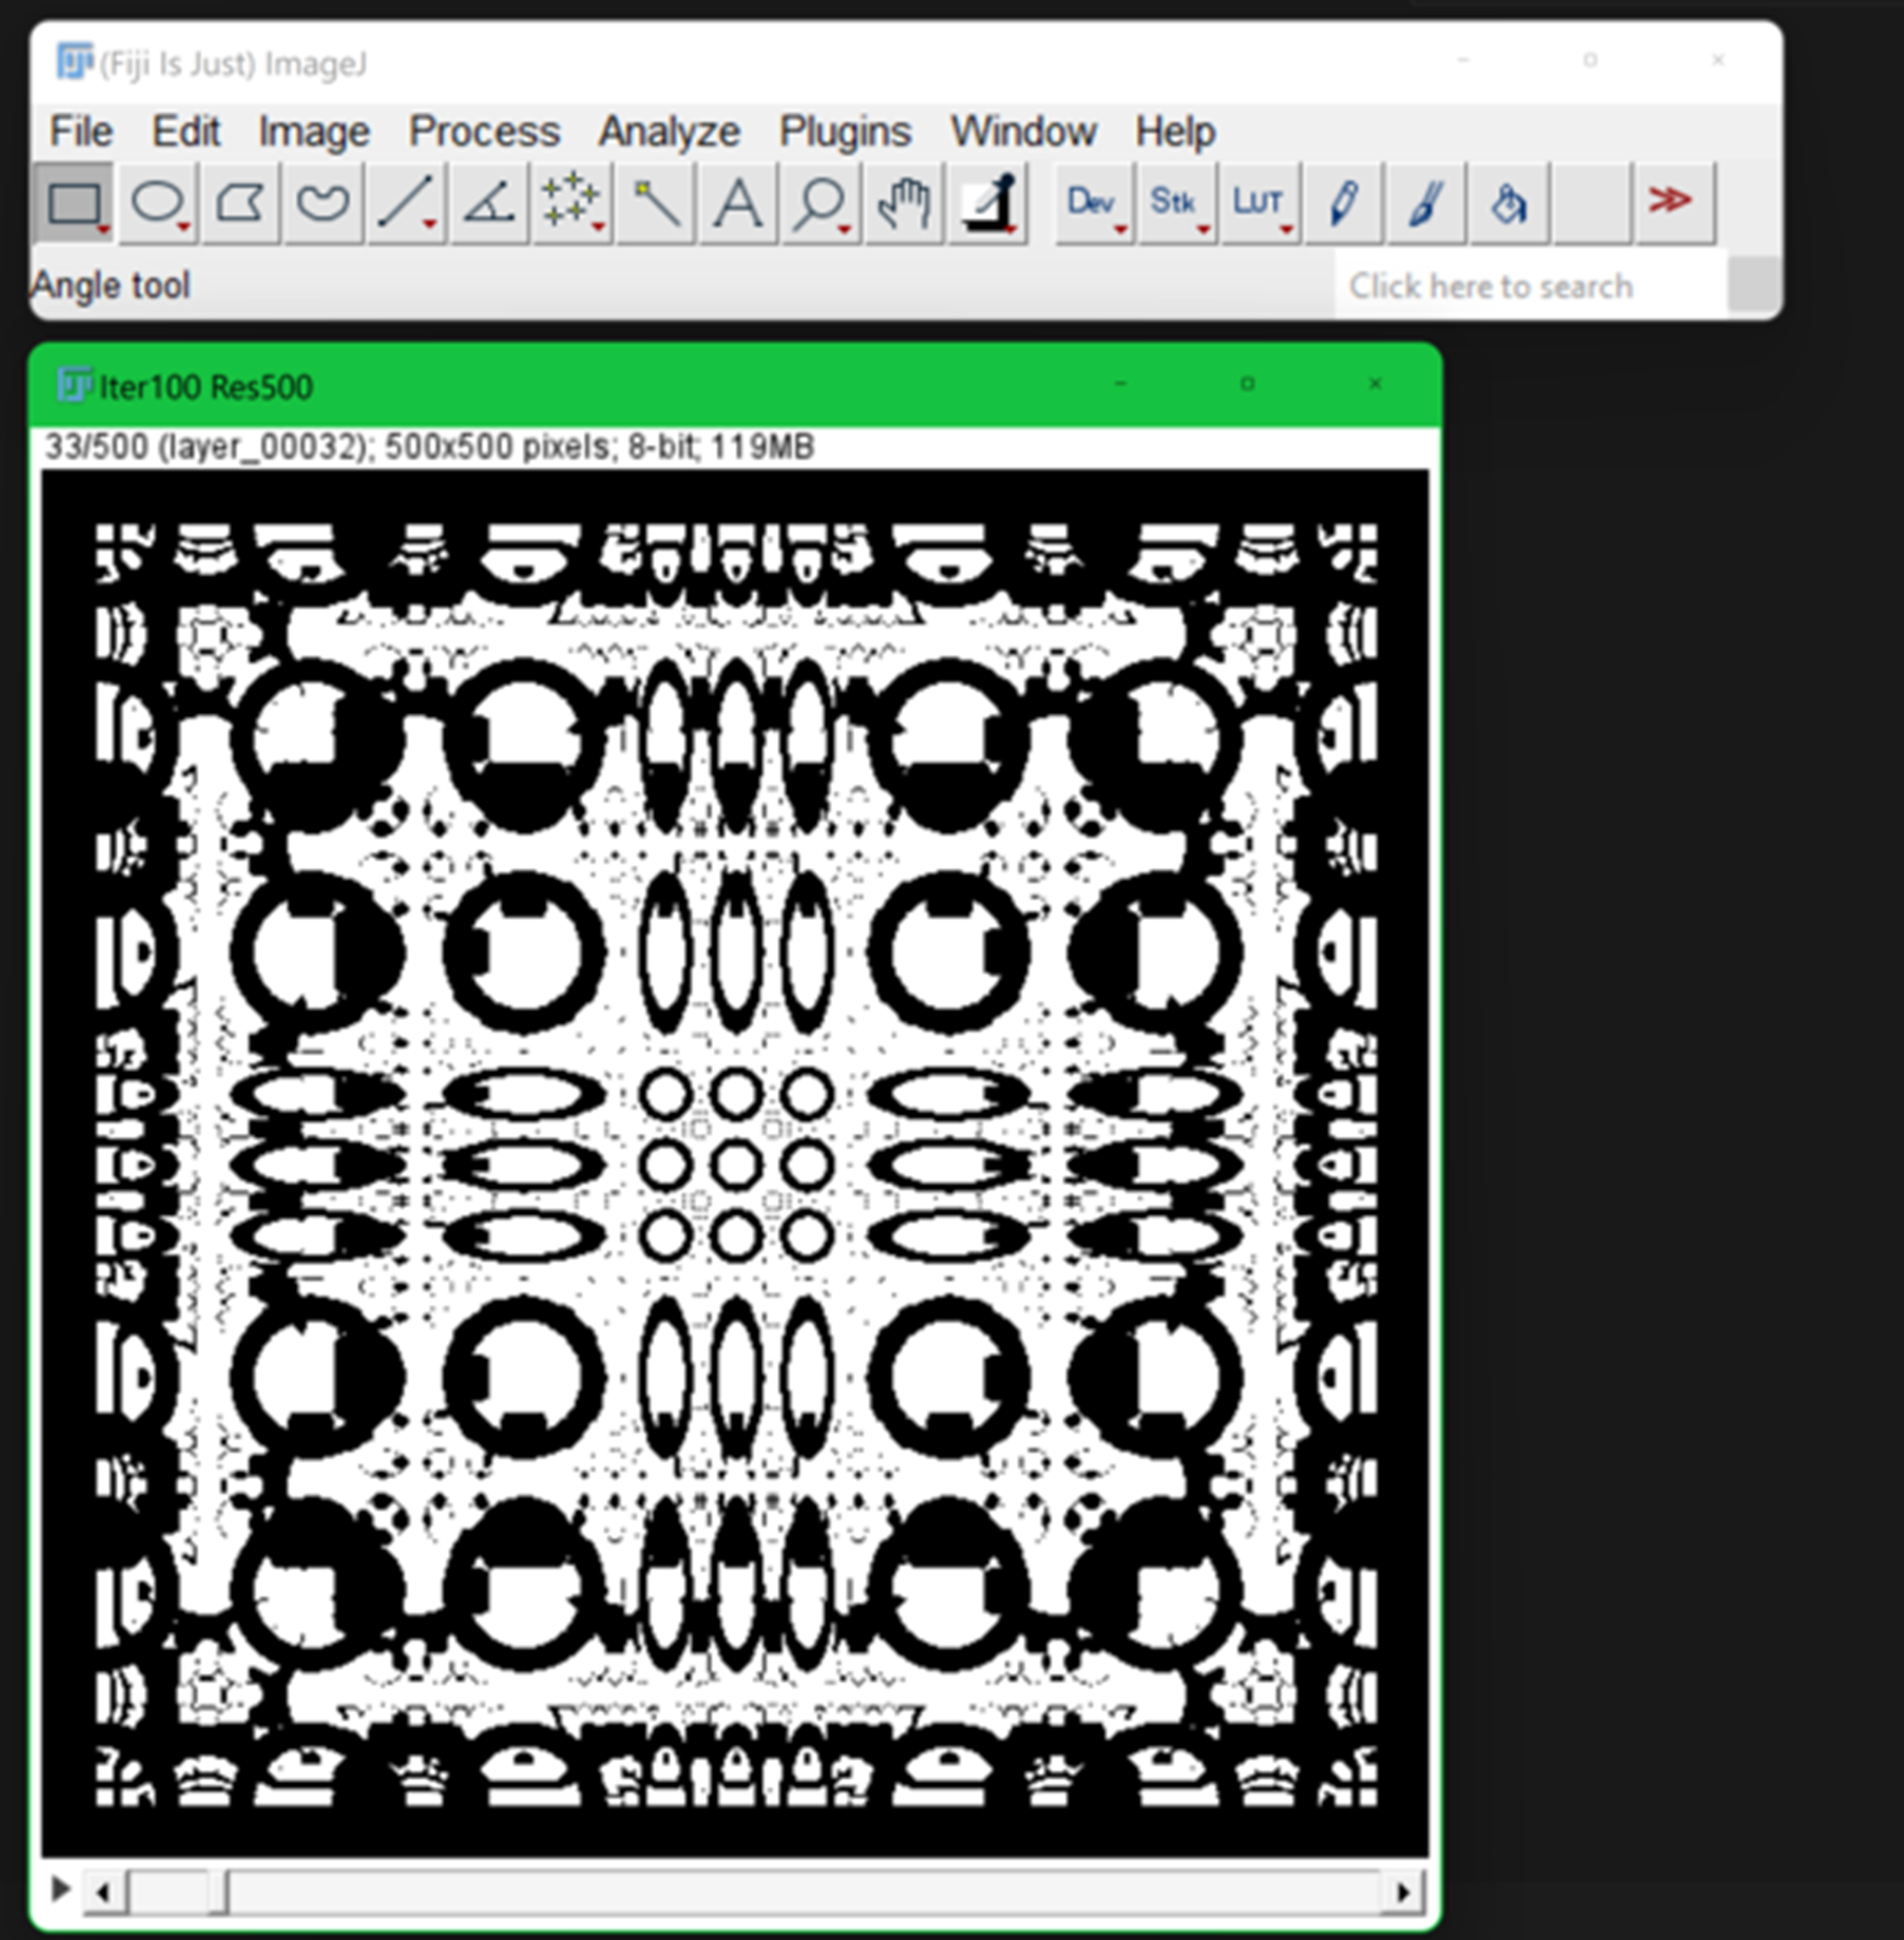
\includegraphics[width=0.8\linewidth]{./images/Picture4.png}
    \caption{Fiji - sukcesor ImageJ}
    \label{fig:fiji}
\end{figure}

Projekt open source oparty o ImageJ2. Oprócz podstawowych operacji wbudowanych w ImageJ posiada też wiele pluginów znacząco rozszerzających możliwości programu. 
Są one skupione na wspomaganiu przetwarzania obrazów skupionych na dziedzinie neurobiologii, ale możliwości są na tyle szerokie, że wiele innych dziedzin nauki z niego korzysta.

Podstawowe działanie programu nie różni się od ImageJ więc, wszystkie jego problemy są też tutaj obecne. Jednakże poprawiona została jego kompatybilność z najnowszymi systemami operacyjnymi.

\subsubsection{GIMP}
\begin{figure}[H]
    \centering
    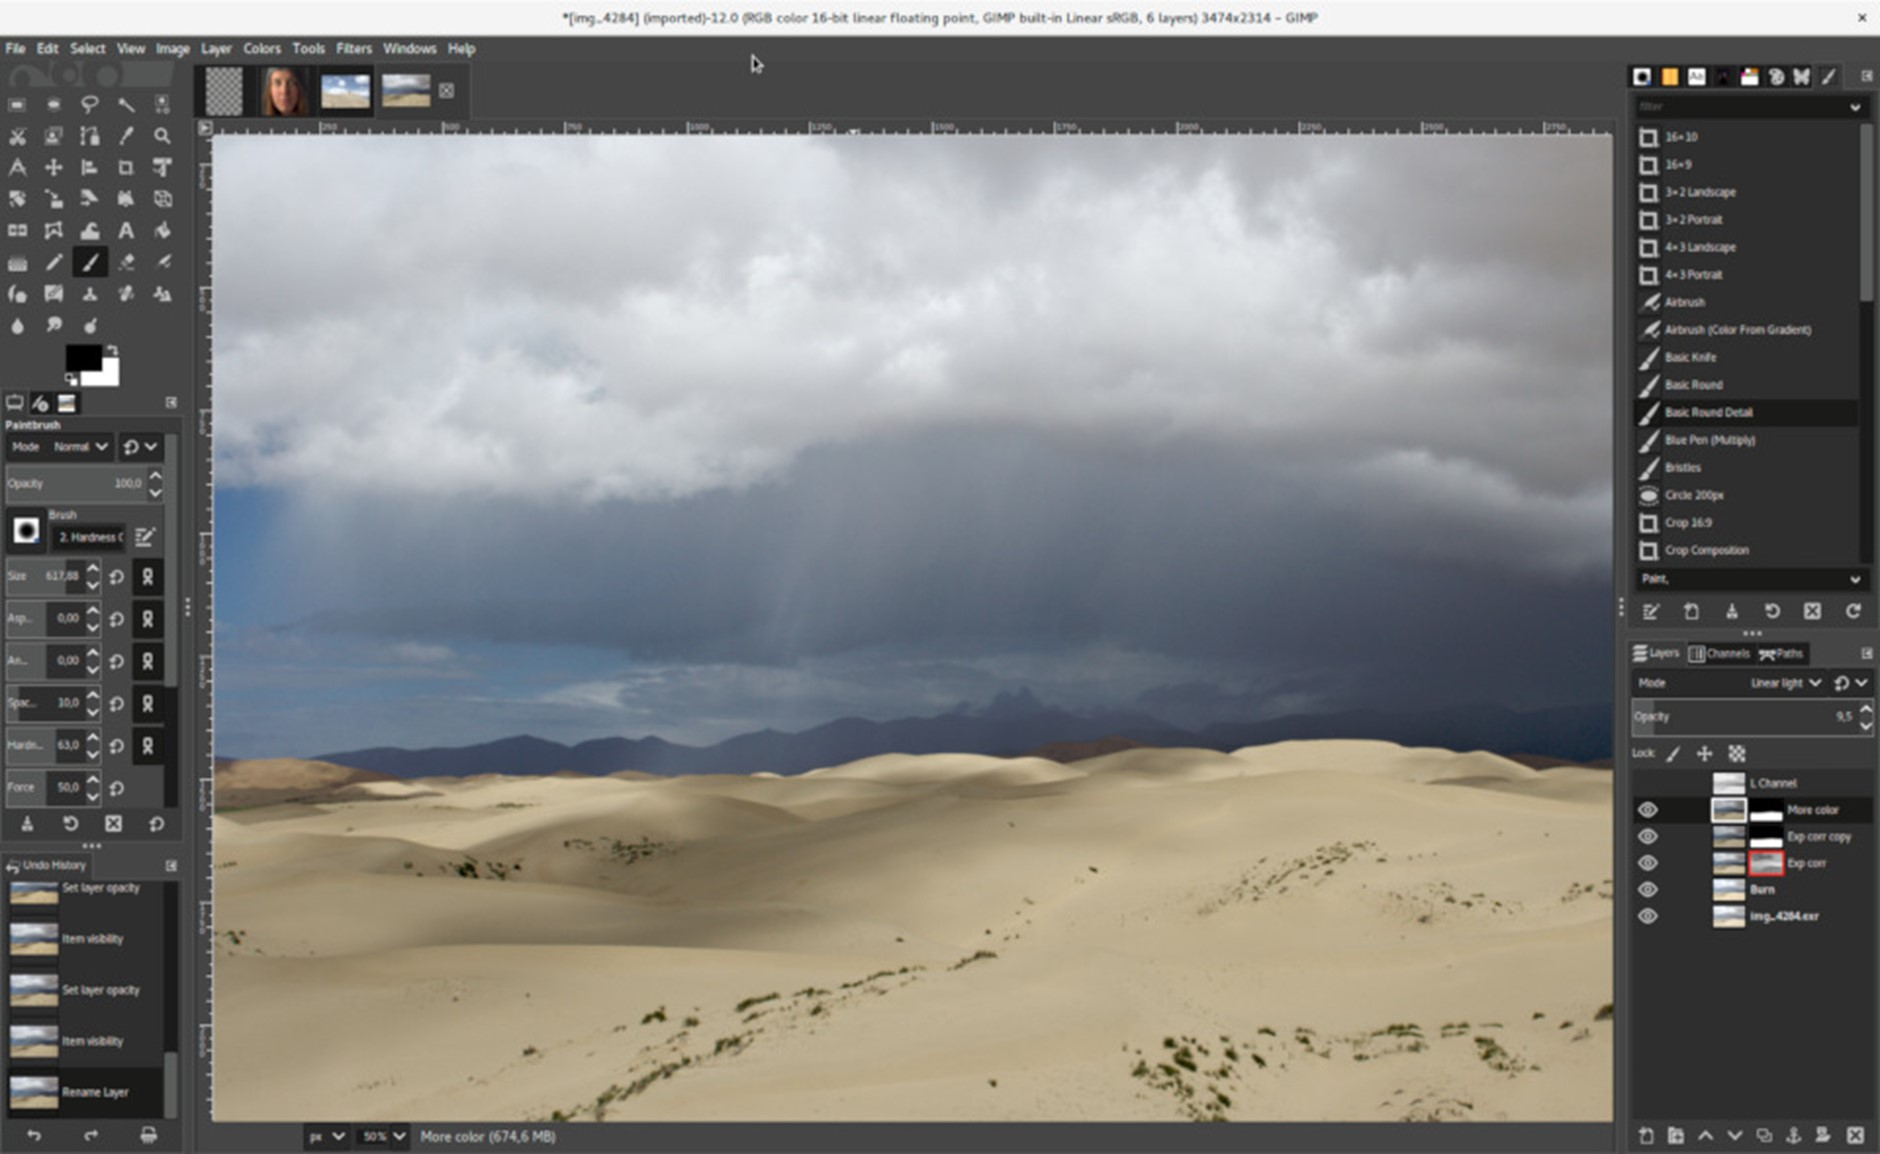
\includegraphics{./images/Picture5.jpg}
    \caption{GIMP wersja 2.10}
    \label{fig:gimp}
\end{figure}

Wydany w 1998 roku GNU Image Manipulation Program jest tworzony jako darmowa konkurencja dla Photoshopa, którego licencja jest miesięczną subskrypcją. Program też w pierwszej kolejności jest tworzony z myślą o artystach, ale posiada więcej zaawansowanych opcji jak np. konwolucje macierzowe które można dowolnie edytować, dając duże możliwości filtrowania obrazów.

Pomimo odwzorowaniu większej liczby operacji ze standardowych bibliotek do przetwarzania obrazów i większej kontroli nad niektórymi z nich nadal występuje problem destruktywnego przetwarzania obrazów. Wynika to z pracy bezpośrednio na obrazie jak w Photoshopie i wymaga szczególnej uwagi przy zarządzaniu warstwami aby nie tracić bezpowrotnie swoich pośrednich operacji w dłuższym ciągu.

\subsubsection{Adobe Substance Designer}
\begin{figure}[H]
    \centering
    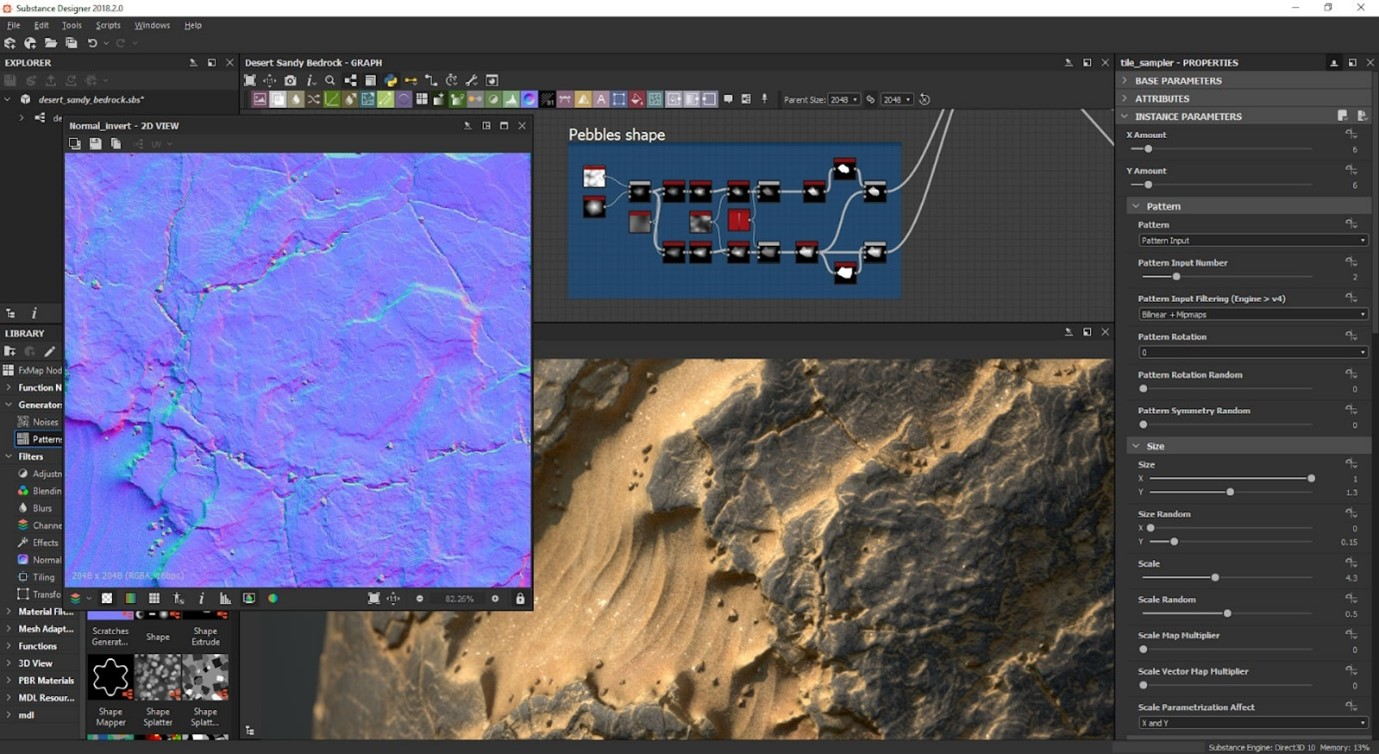
\includegraphics{./images/Picture6.jpg}
    \caption{Adobe Substance Designer}
    \label{fig:designer}
\end{figure}

Wydany w 2007 roku program był główną inspiracją dla tego projektu. 
Jego dużą zaletą jest to, że tworzenie algorytmów bazuje na układaniu bloczków (nodów). 
Ułożony graf jest wykonywany na obrazie, który importujemy do programu lub generujemy go od początku w nim. 
Każdy dowolny node można kliknąć i zmienić wszystkie parametry jego operacji, niezależnie w którym miejscu ciągu znajduje się.
Jego wynik i wszystkie następne operacje, które są zależne od niego są obliczane ponownie na podstawie zmienionego wyniku. 
Zmiana przetwarzanego obrazu polega na przeciągnięciu połączenia z obecnego węzła z naszym plikiem wejściowym na nowy bloczek. Następnie propagowana jest zmiana na wszystkie kolejne operacje, których wynik jest aktualizowany automatycznie.

Opisywany program ten ma wiele ograniczeń związanych z tym, że nie jest stworzony do ogólnego przetwarzania obrazów. Został natomiast stworzony do tworzenia materiałów/tekstur do grafiki komputerowej. 
Obrazy są ograniczone do boków o długości $2\textsuperscript{n}$, najlepiej kwadratowych. 
Parametry operacji są często uproszczone, ponieważ mimo większej złożoności aplikacji, jest ona nadal skierowana do artystów. 
Rodzaje operacji i wspierane formaty pikseli w pliku są przystosowane do wymagań grafiki komputerowej.

\newpage

\section{Zakres użytych technologii i opis wykorzystywanych narzędzi}
Wybór technologii ma duży wpływ na różne aspekty projektu programistycznego.
Od niego zależy na jakich platformach może zostać on tworzony i uruchamiany.
Dobre biblioteki potrafią znacząco ułatwić tworzenie oprogramowania pozwalając skupić się programistom na tworzeniu funkcjonalności aplikacji.
Nie ma potrzeby tworzyć nowego systemu wyświetlania interfejsu użytkownika na potrzebę każdego projektu osobno, gdy jest wybór wielu bardzo dobrze wspieranych technologii na każdą platformę.

Przy wyborze technologii dla aplikacji oprócz funkcjonalności zostały wzięte pod uwagę:
\begin{itemize}
    \item \textbf{Dobrze napisaną dokumentację:} Obsługa biblioteki programistycznej jest dużo łatwiejsza, gdy jej twórca udostępnia dobrze napisane materiały jak z niej korzystać.
    \item \textbf{Otwarty kod źródłowy:} Projekty open source udostępniają swój kod - nawet w momencie, kiedy dokumentacja nie jest idealna możemy zobaczyć jak dana funkcja działa.
    \item \textbf{Aktywne utrzymywanie:} Biblioteka bez aktualizacji do nowszych wersji może sprawiać problemy w postaci luk bezpieczeństwa lub problemami z kompatybilnością.
    \item \textbf{Dojrzała technologia:} Korzystając z kodu tworzonego i używanego od wielu lat można spodziewać się większej ilości przykładowych użyć, dopracowanego interfejsu projektu oraz pozbawionego błędów działania.
\end{itemize}

\subsection{Język programowania}

Jest to kluczowy wybór, ma wpływ na większość następnie wybranych technologii.
Język programowania ma wpływ na wydajność aplikacji, trudność jej tworzenia oraz późniejszego utrzymania.
Dzięki wyborze popularnego języka można mieć dostęp do bardzo szerokiej gamy gotowych bibliotek rozwiązujących popularne problemy jak komunikacja z serwerami czy zapisywanie i odczytywanie formatu JSON.

\subsubsection{C\#}

Wieloparadygmatowy język ogólnego przeznaczenia tworzony przez Microsoft od ponad 20 lat \cite{csharp}.
Jest on kompilowany przed uruchomieniem co daje przewagę wydajności nad językami interpretowanymi.
Można obecnie pisać w nim aplikacje na komputery stacjonarne, telefony, przeglądarki czy serwery.
Posiada narzędzie do zarządzania bibliotekami NuGet \cite{nuget} pozwalająca na łatwe dodanie zależności do projektu.

\subsection{Platforma programowa}

Wiele języków programowania posiada swoją platformę programistyczną - jest to narzędzie za pomocą którego można tworzyć projekty, zarządzać bibliotekami, budować i uruchamiać aplikację.

\subsubsection{.NET Core}

.NET Core to platforma programistyczna opracowana przez firmę Microsoft, stanowiąca otwartoźródłowe i wieloplatformowe środowisko do tworzenia różnorodnych typów aplikacji, w tym aplikacji internetowych, usług sieciowych oraz aplikacji konsolowych.
Obsługuje wiele języków z których najpopularniejszy jest C\# \cite{dotnet}.
Jej struktura podzielona jest na moduły takie jak środowisko uruchomieniowe, kompilacja czy wbudowane biblioteki.

\subsection{Interfejs użytkownika}

W celu zapewnienia użytkownikom szybkiego wykonywania operacji wybrano jako docelową platformę komputer stacjonarny.
Zawęża to wybór możliwych technologii tworzenia interfejsu.
Rozważone zostały dwie technologie - Avalonia UI \cite{AvaloniaUI} oraz WPF \cite{wpf}.
Pierwsza z nich jest nowsza i aktywnie rozwijana, może działać na wielu platformach w przeciwieństwie do rozwiązania stworzonego przez Microsoft. 
W momencie decydowania o interfejsie użytkownika jednak pojawiały się błędy w funkcjonalnościach potrzebnych do działania projektu.

\subsubsection{Windows Presentation Foundation}

Jest to platforma graficzna opracowana przez firmę Microsoft, została po raz pierwszy wprowadzona jako część .NET Framework w 2006 roku \cite{wpfHistory}. 
Umożliwia tworzenie bogatych interfejsów użytkownika dla aplikacji stworzonych na system Windows.
Elementy są wyświetlane wektorowo co pozwala na dowolne skalowanie elementów. 
Widoki są definiowane w formacie XAML co pozwala na oddzielenie logiki biznesowej od warstwy prezentacji.
Platforma ta umożliwia powiązanie elementów interfejsu z danymi aplikacji co pozwala na szybkie aktualizowanie widoku z najnowszymi wynikami.

\subsubsection{Nodify}
\begin{figure}[H]
    \centering
    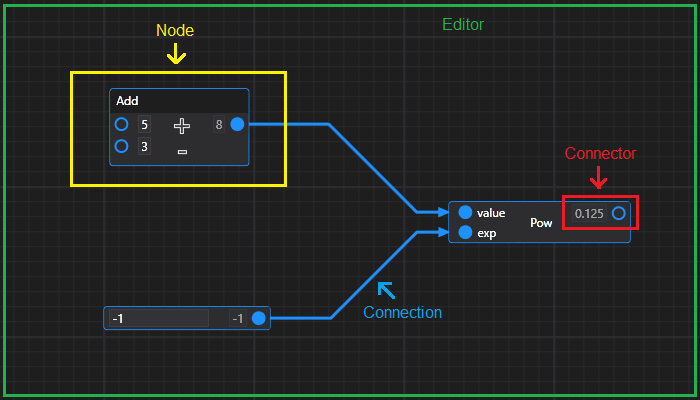
\includegraphics[width=0.8\linewidth]{./images/Picture7.png}
    \caption{Opis elementów edytora węzłów \cite{node}.}
    \label{fig:nodify}
\end{figure}

Biblioteka Nodify \cite{nodify} jest otwartoźródłowym projektem implementującym edytor węzłowy \autoref{fig:nodify} dla biblioteki WPF. 
Poprawna implementacja tego projektu daje możliwość dodawania bloczków i łączenie ich w ciągi. 
Wystarczy zaimplementować co dzieje się z danymi w węzłach oraz jak zostają one przekazywane dalej żeby mieć funkcjonalny interfejs użytkownika. 

\subsubsection{WPF UI}
\begin{figure}[H]
    \centering
    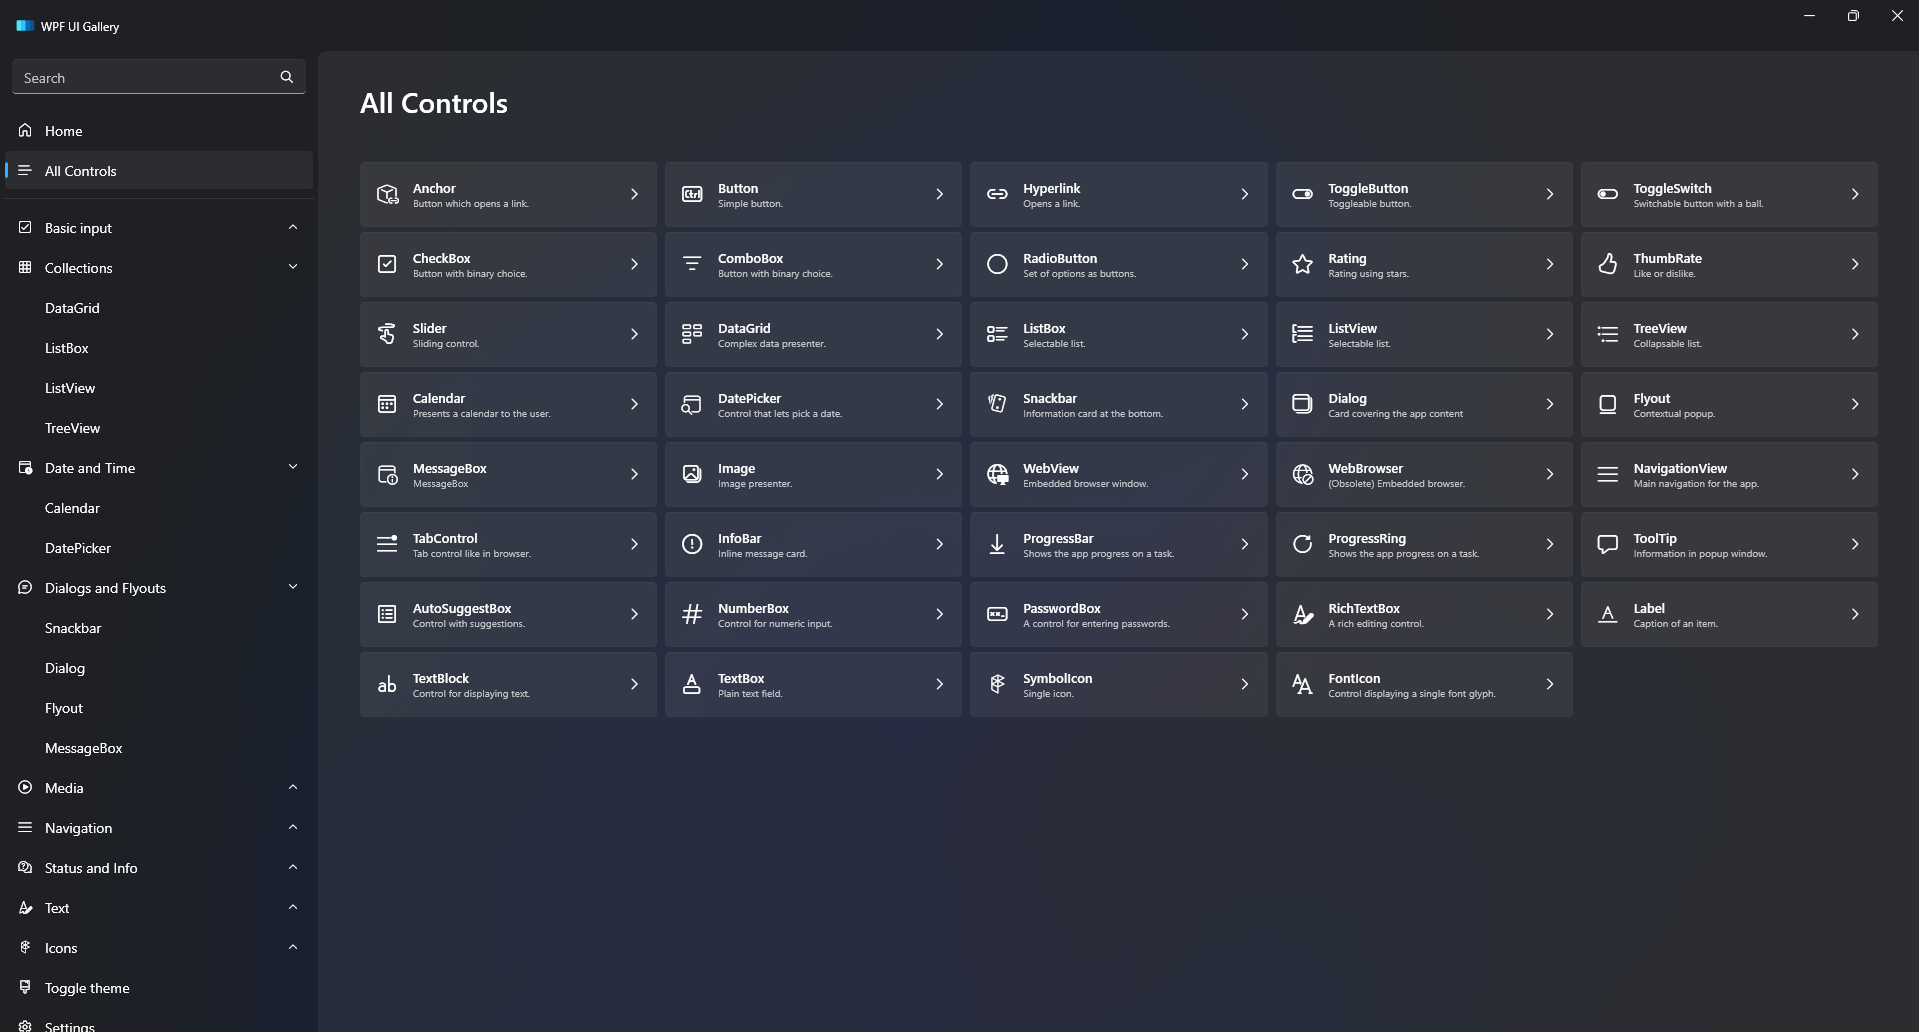
\includegraphics[width=0.9\linewidth]{./images/Picture8.png}
    \caption{Galeria elementów WPF UI. Opracowanie własne.}
    \label{fig:wpfui}
\end{figure}

Biblioteka WPF UI \cite{wpfui} modyfikuje i dodaje elementy interfejsu używane w Windows Presentation Foundation \autoref{fig:wpfui}. 
Jest ona zgodna z systemem projektowania interfejsu Fluent 2 \autoref{fig:winui3} od Microsoftu używanego w wielu aplikacjach dla systemu Windows 11. 
Pozwala to na utrzymanie nowoczesnej stylistyki w projekcie bez potrzeby tworzenia skomplikowanych stylów imitujących WinUI 3 od zera.

\begin{figure}[H]
    \centering
    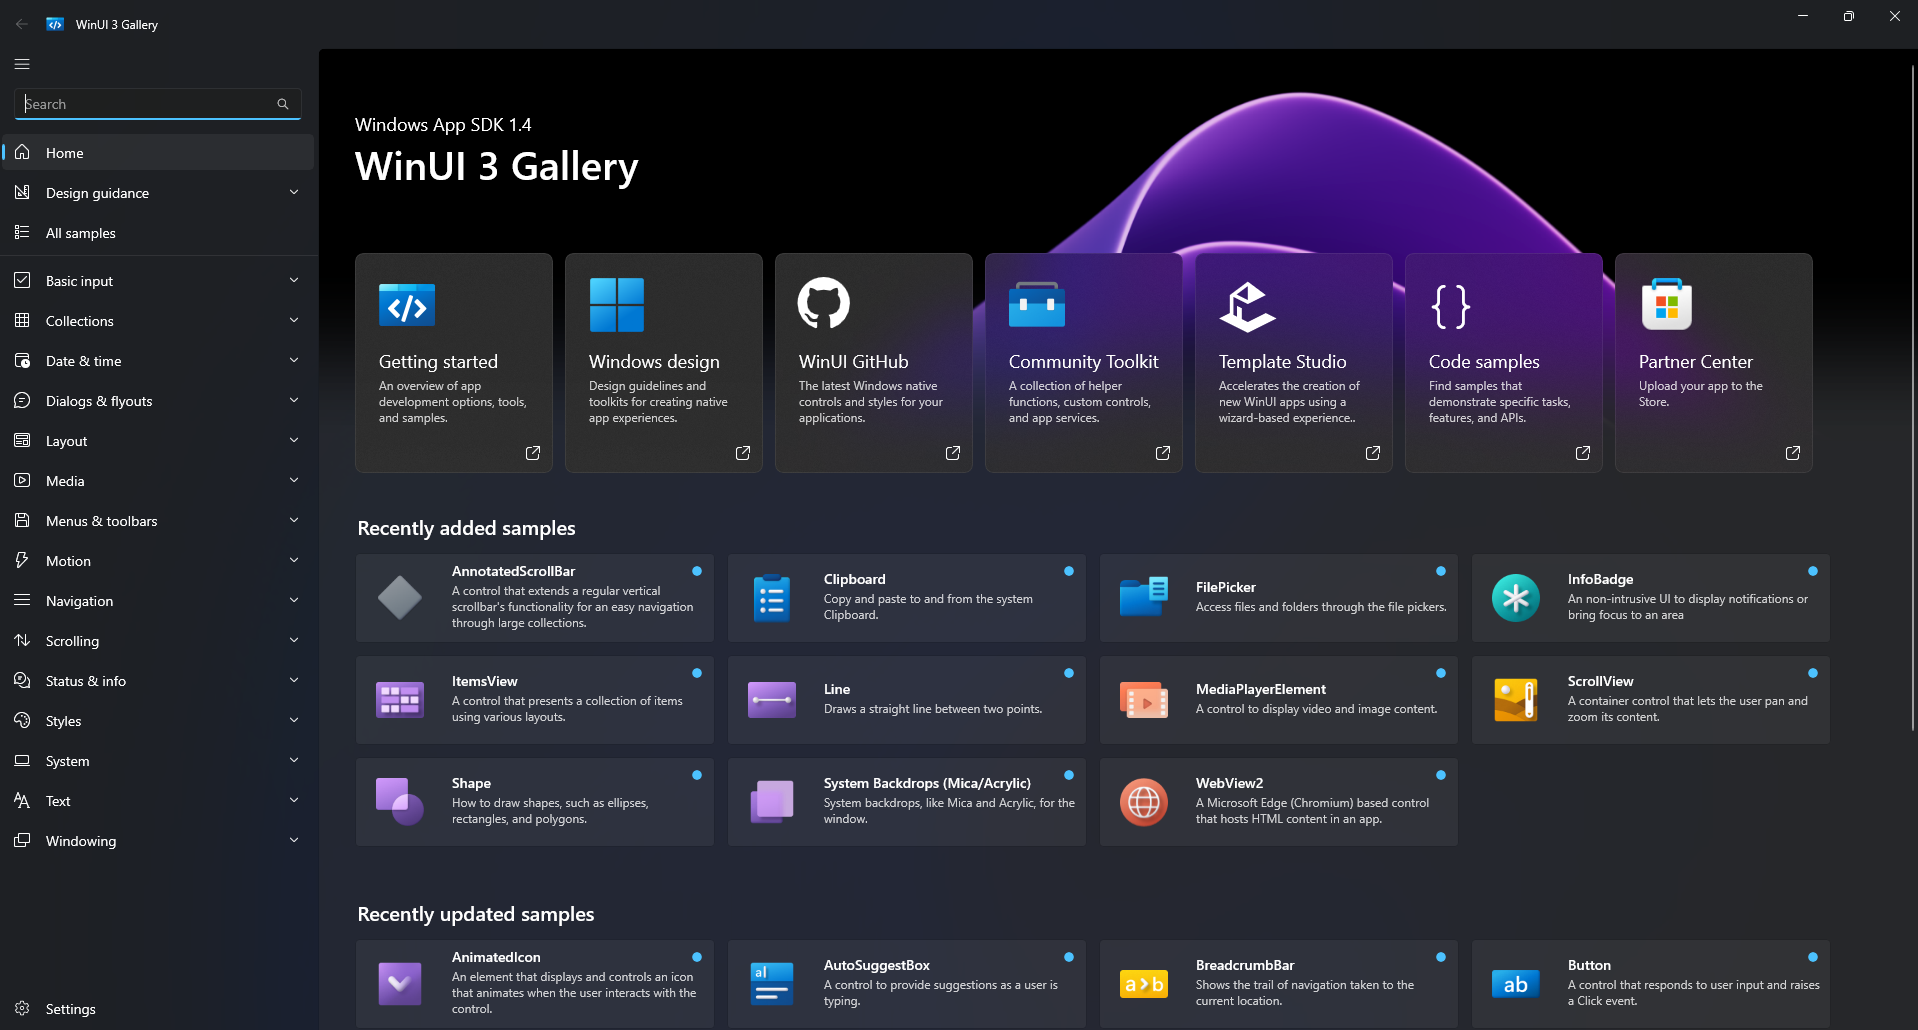
\includegraphics[width=0.9\linewidth]{./images/Picture9.png}
    \caption{Galeria elementów WinUI 3. Opracowanie własne.}
    \label{fig:winui3}
\end{figure}

\subsection{Biblioteka do przetwarzania obrazów}
Jedną z popularnych bibliotek do przetwarzania obrazów jest OpenCV.
Nazwa to skrót od \textit{Open Source Computer Vision Library} i wskazuje, że jest to darmowy i otwartoźródłowy projekt skupiony na przetwarzaniu obrazów oraz widzeniu maszynowym.
Pakiet ten dostępny jest dla systemów Windows, macOS i Linux. 
Został stworzony w Intel Research Labs w 1999 roku \cite{opencvHistory}. Biblioteka ta jest napisana w języku C\++ i kładzie duży nacisk na prędkość obliczeń. Pozwala ona na przetwarzanie obrazów, wideo, posiada zaawansowane algorytmy wykrywania obiektów, klasyfikacji oraz wiele operacji korzystajacych z sieci neuronowych.

\subsubsection{OpenCvSharp}

Projekt jest tworzony w języku C\# więc nie możemy bezpośrednio odwoływać się do biblioteki OpenCV. Powstało kilka projektów które opakowują oryginalny pakiet w metody którymi możemy się odwołać bez problemu z kodu w platformie .NET. Dwie najpopularniejsze biblioteki tego typu to EmguCV \cite{emgucv} oraz OpenCvSharp \cite{opencvsharp}. 
Obie cieszą się dużym wsparciem społeczności lecz pierwsza z nich jest mniej zgodna z API oryginalnej paczki oraz jest wolniejsza.

\subsection{Biblioteka do walidacji}

W interfejsie użytkownika należy wprowadzić dane, nie możemy założyć że będą one poprawne.
Wszystkie wejścia trzeba zabezpieczyć tak by użytkownik nie mógł przerwać działania programu i zawsze wiedział dlaczego jego operacje się nie wykonują.

\subsubsection{Fluent Validation}

Biblioteka Fluent Validation \cite{fluentvalidation} pozwala na proste ustalanie reguł według których ocenia czy dane są prawidłowe oraz przypisanie odpowiedniej wiadomości błędu gdy nie są. Paczka ta jest przejrzysta oraz posiada dobrą dokumentację i wiele przykładów implementacji. 

\subsection{Biblioteka do serializacji}

Serializacja jest potrzebna gdy chcemy zapisać stan naszej aplikacji lub wysłać jakieś dane. Dla wygody użytkownika należy wprowadzić system zapisywania i wczytywaniu plików, żeby mógł wrócić do wcześniej stworzonych ciągów operacji oszczędzając jego czas. 

\subsubsection{Json.NET}

Newtonsoft.Json \cite{Newtonsoft.Json} to najpopularniejsza biblioteka do obsługi plików Json w galerii paczek NuGet \cite{jsonMostPop}. 
Pozwala na serializowanie obiektów i deserializowanie Json'a do obiektów zachowując złożone struktury obiektów i kolekcje oraz posiada wiele parametrów za pomocą których można dopasować jego wyniki do większości zastosowań. 

\subsection{Środowisko deweloperskie}

Odpowiednie środowisko może znacząco przyśpieszyć pracę nad projektem programistycznym. 
Nowoczesne IDE (ang. \textit{Integrated Development Environment}) zamykają nawiasy, pomagają w poprawianiu błędów, refaktoryzacji i proponują automatyczne uzupełnienia zmiennych czy metod biorąc pod uwagę kontekst kodu w plikach.
Ważne jest też zadbanie o kontrolę wersji w celu zapisywania stanu projektu oraz śledzeniu zmian zachodzących w nim.

\subsubsection{Microsoft Visual Studio}
\begin{figure}[H]
    \centering
    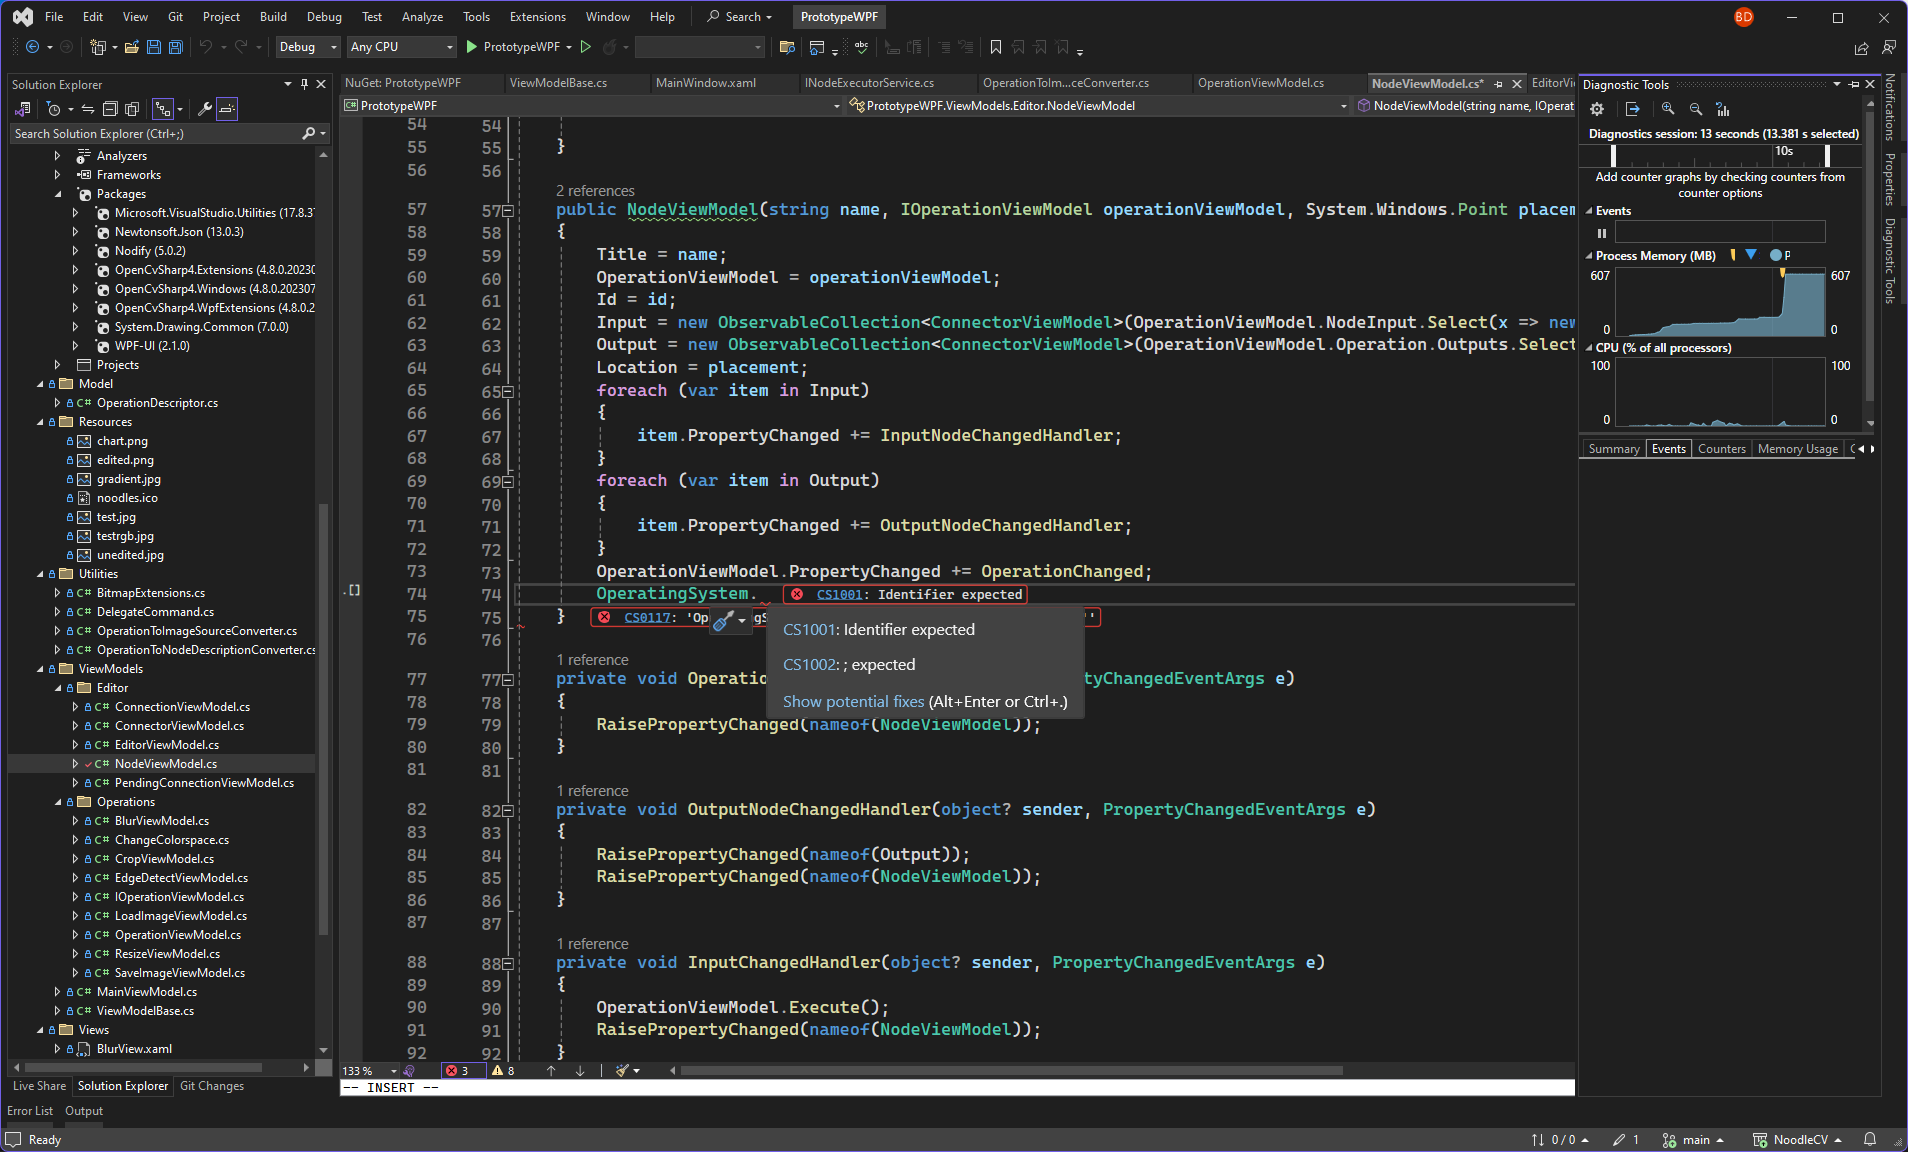
\includegraphics[width=1\linewidth]{./images/Picture10.png}
    \caption{Interfejs programu Visual Studio. Opracowanie własne.}
    \label{fig:visual}
\end{figure}

Microsoft Visual Studio \cite{visualstudio} to zintegrowane środowisko programistyczne (IDE) opracowane i wydane przez firmę Microsoft. Jest przeznaczone do tworzenia aplikacji komputerowych, w tym aplikacji internetowych, aplikacji mobilnych, aplikacji desktopowych i aplikacji konsolowych. Posiada wiele gotowych zestawów narzędzi do pobrania dla specyficznych typów programów, a jego funkcjonalność dodatkowo można rozszerzać dodatkami pobieranymi z internetu.

\subsubsection{Git}

Git \cite{git} to system kontroli wersji oparty na rozproszeniu danych (ang. \textit{distributed version control system - DVCS}), opracowany przez Linusa Torvaldsa. 
Jest przeznaczony do śledzenia zmian w plikach i folderach, a także do współpracy nad projektami w czasie rzeczywistym. 
\newpage

\section{Realizacja projektu}
\subsection{Zastosowania}
\begin{itemize}
    \item \textbf{Tworzenie gotowych ciągów operacji:} Czasem potrzebne jest przetworzenie małej ilości obrazów, lub problem jest na tyle mało skomplikowany, że nie ma sensu szukać programisty, który stworzy dla nas program, ale bez wiedzy o programowaniu zrobienie tego w kodzie samodzielnie może być zbyt ciężkie. Program z interfejsem graficznym pozwoli na stworzenie procesów nawet przez osoby mniej techniczne.
    \item \textbf{Uczenie się:} Osoby chcące poznać techniki przetwarzania obrazów będą mogły w prosty sposób bez znajomości programowania zobaczyć na własne oczy działanie funkcji, ich interakcję ze sobą oraz łatwo dopasowywać ich parametry. 
    \item \textbf{Komunikacja:} Dzięki temu oprogramowaniu programista może łatwiej i efektywniej porozumieć się z osobami mniej zaznajomionymi z programowaniem i dużo szybciej wprowadzać zmiany w porównaniu z pisaniem kodu i jego kompilacją przy każdej zmianie.
\end{itemize}
\subsection{Wymagania funkcjonalne i niefunkcjonalne}
Oprogramowanie opisane w tej pracy to \textbf{NoodleCV}. 
Następne podrozdziały przedstawią wymagania z jakimi trzeba było się zmierzyć w trakcie tworzenia aplikacji.
\subsubsection{Wymagania funkcjonalne}
Wymagania funkcjonalne?
\begin{itemize}
    \item Przetwarzanie obrazów
\end{itemize}
\subsubsection{Wymagania niefunkcjonalne}
Niefunkcjonalne wymagania?
\begin{itemize}
    \item Łatwość użytkowania
\end{itemize}
\newpage

\section{Podsumowanie}
Celem pracy było stworzenie aplikacji do przetwarzania obrazów z interfejsem graficznym.
Interakcja użytkownika z programem odbywa się przez edytor węzłowy, a parametry odpowiadają tym używanym w bibliotece OpenCV. 
Wyniki obliczeń zostają wyświetlane natychmiastowo, a parametry które można wprowadzić są sprawdzane pod kątem poprawności.  
Cel został zrealizowany.

Projekt jednak ma duży potencjał na rozwój. Inspirując się innymi projektami z podobnymi edytorami można wymienić całą listę: 
\begin{itemize}
    \item tworzenie i zapisywanie parametrów do użycia jak zmienne w programowaniu - zmiana wartości w jedynym miejscu zmienia też jej użycia w innych operacjach,
    \item możliwość łączenia kilku bloków w jeden przez użytkownika np. \textit{Blur} i \textit{EdgeDetect} ponieważ są one często używane razem,
    \item grupowanie, układanie i komentarze w edytorze,
    \item miniaturka z podglądem wyniku umieszczona na każdym węźle,
    \item eksportowanie pliku w sposób pozwalający zmianę parametrów i podgląd wyników przez zewnętrzny program.
\end{itemize}

OpenCV jest bardzo obszerną biblioteką z racji czego projekt został ograniczony do prostych operacji. Obszary do poprawy to:
\begin{itemize}
    \item zwiększenie liczby metod przetwarzania obrazów dostępnych w aplikacji,
    \item wsparcie dla innych typów danych jak wideo, chmury punktów itd.,
    \item użycie funkcji korzystających z sieci neuronowych czy uczenia maszynowego,
    \item wybór metody gdy więcej niż jedna realizuje ten sam cel.
\end{itemize}

Obecnie program działa tylko na komputerach z systemem Windows, wprowadzenie wsparcia dla uruchamiania na innych platformach pozwoli na zwiększenie potencjalnej liczby użytkowników. Do rozważenia jest skorzystanie z obliczeń w chmurze - nie każdy posiada wystarczająco szybkie urządzenia, a jako bonus użytkownicy mobilni czy systemów wbudowanych (ang. \textit{embedded systems}) też mogli by korzystać z aplikacji z zadowalającymi osiągami. 
\newpage
\newpage

\addcontentsline{toc}{section}{Bibliografia}
\printbibliography % https://www.overleaf.com/learn/latex/Bibliography_management_in_LaTeX#Reference_guide

\newpage

\addcontentsline{toc}{section}{Spis rysunków}
\listoffigures
\newpage

\addcontentsline{toc}{section}{Spis tabel}
\listoftables
\newpage

\addcontentsline{toc}{section}{A. Załączniki}
\section*{A. Załączniki}
\input{sections/attachments}
\end{document}